\documentclass{article}
\usepackage{graphicx} % Required for inserting images
\usepackage{multicol}
\usepackage{hyperref}
\graphicspath{{images/}} % configuring the graphicx package
\title{ACTORS DETECTION AND RETRIEVAL IN MOVIE SCENES}
\author{Bianco Michael, Bertolini Matteo, Todaro Marco}
\date{May 2023}

\begin{document}
\maketitle
\section{Introduction}

Our idea is to build a deep learning algorithm to recognize and detect celebrities acting in different 
movie scenes, 
even if they are dressed up, made up or in movement.
The literature necessary to work on this kind of model requires the study of convolutional neural networks
for extracting the most salient features useful to describe each actor we are recognizing and algorithms for edge
detection, in particular for face detection.

\begin{center}
\begin{multicols}{2}
\vspace*{-0.4in}
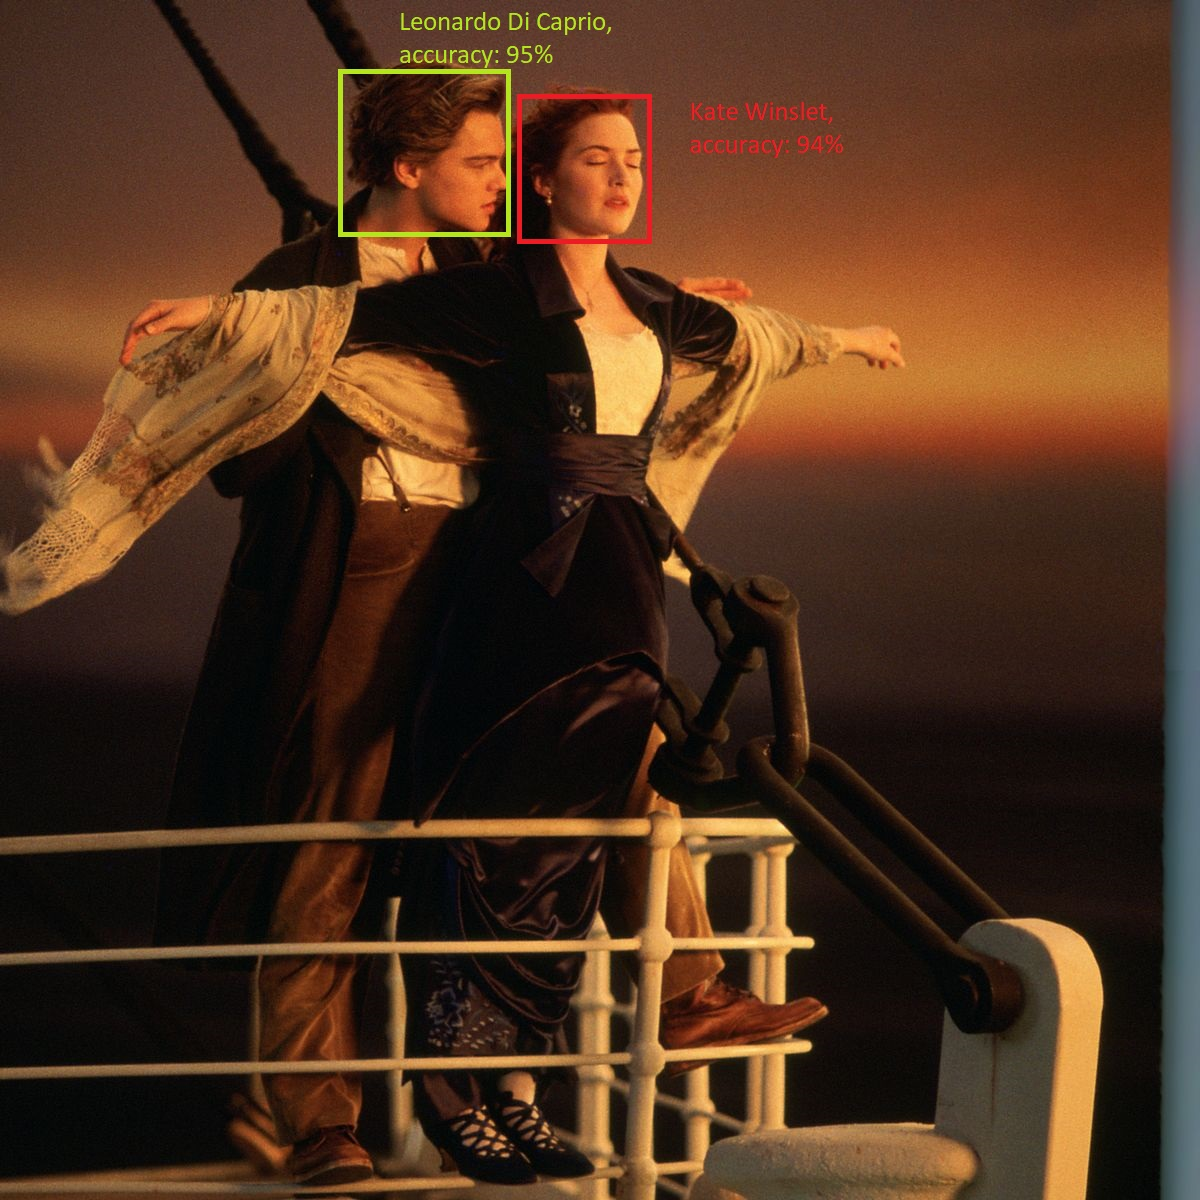
\includegraphics[scale=0.33]{intro1.jpeg}  
\hspace*{.4in}
{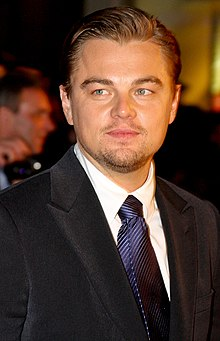
\includegraphics[scale=0.32]{intro3.jpeg}} 
\\
\hspace*{.4in} 
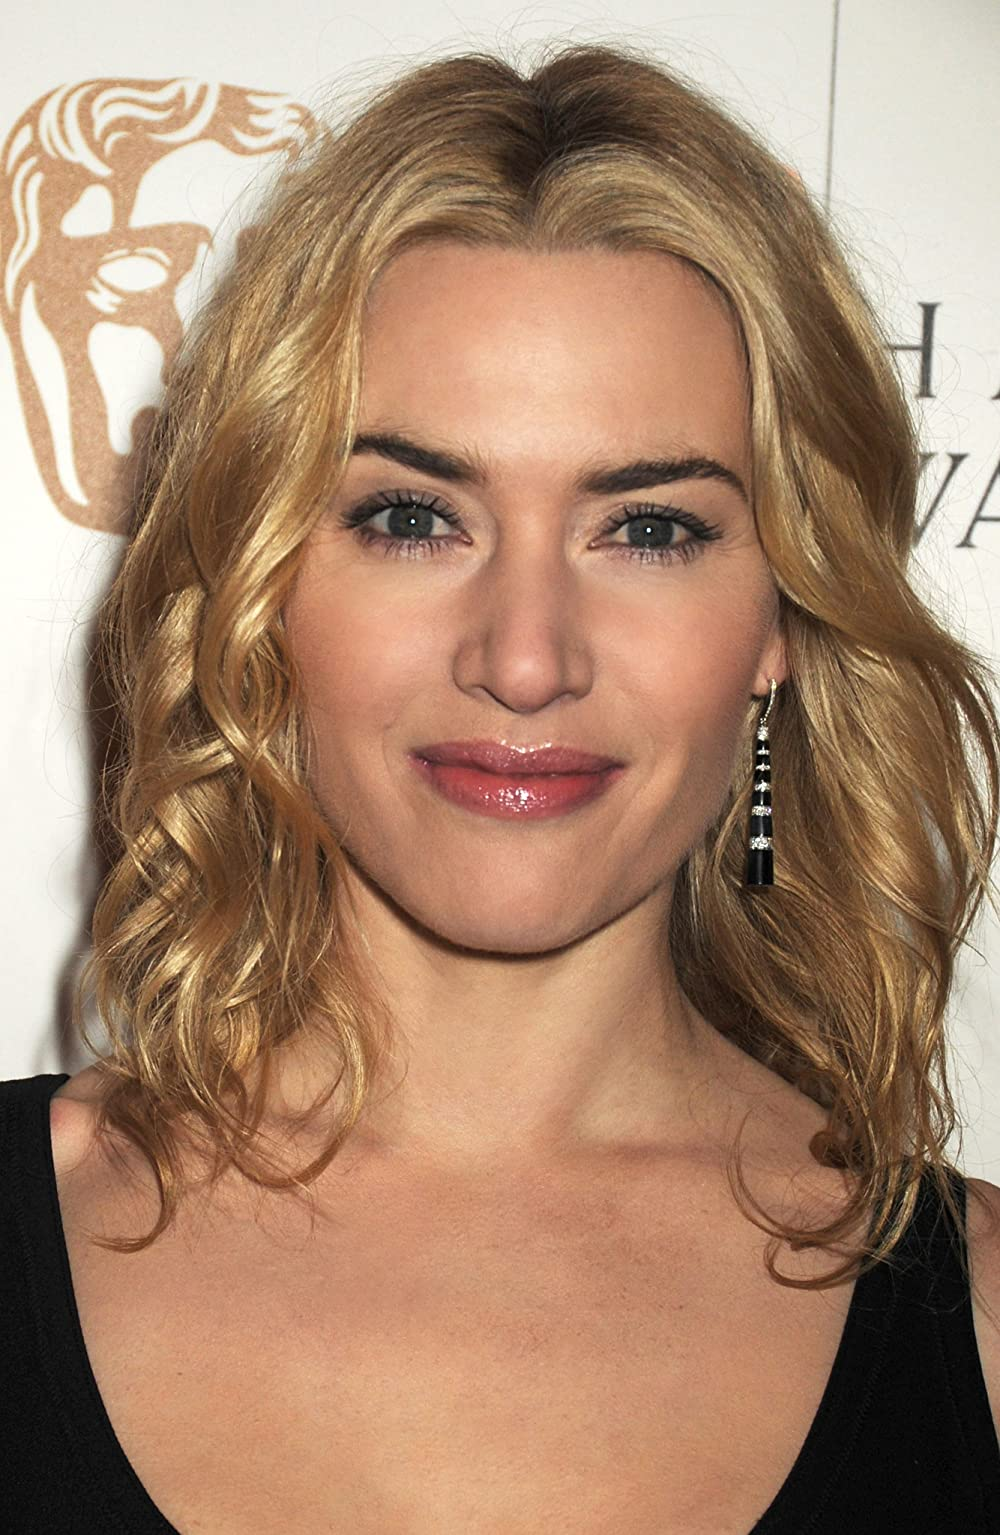
\includegraphics[scale=0.07]{intro2.jpeg}  
\end{multicols}
\end{center}
\vspace*{0.2in}

\section{Problem statement}
The dataset of actors is made of 20 images per 16 celebrity (12 used for train and 8 for test), for a total of 320 images.
\\The actors are : 
Anne Hathaway,
Anthony Hopkins,
Brad Pitt,
Claire Forlani,
Demi Moore,
Denzel Washington,
Johnny Depp,
Kate Winslet,
Leonardo DiCaprio,
Margot Robbie,
Matt Damon,
Matthew McConaughey,
Morgan Freeman,
Robert DowneyJR,
Scarlett Johansson,
Tom Cruise.\\\\
Steps towards the goal:
\begin{itemize}
  \item Create our own dataset of actor faces, labelled with their name
  \item Process the images with filters and resize them all to the same dimensions
  \item Starting from VggFace weights, fine tune the network on the last three fully-connetected layers
  \item Apply dropout and some heuristics to reach an accuracy higher than 90\% during training on our dataset
  \item Starting from a video, for each possible frame use yoloface to detect the faces of the actors, use some geometry
  \item Given a frame and the bounding boxes of the faces, classify the correct names for the actors in the scene.
  \item Retrieval: provide additional photos and information about the actors founded.
\end{itemize}

\section{Technical Approach}
In order to build the dataset, we take original images from the web, organized in directories named with the name of the actor,
extract the first 12 images, resize them to (224,224) and assign each of them to the TRAIN set.
The same is done for the other 8 images, assigned to the TEST set.
\\\\
Starting from the weights for VggFace available at \url{https://www.robots.ox.ac.uk/}, 
we rewrote the VGG FACE network pre-trained with LFW dataset.
\\\\
The last layer has been modified to 16 output parameters in order to classify with the actors in our dataset,
Then we performed a fine-tuning of the last three layers FC (almost 120M parameters) and saved final weights.
\\
To integrate our model with the face-detection algorithm, we loaded the trained network in a script, then extracted each frame from a video
and performed face detection with yoloface.
For each face detected, forwarded it to the network and draw a rectangle around the face with the prediction of the actor name,
in the end reconstruct the video.
\\ 

\section{Intermediate/Preliminary Results}
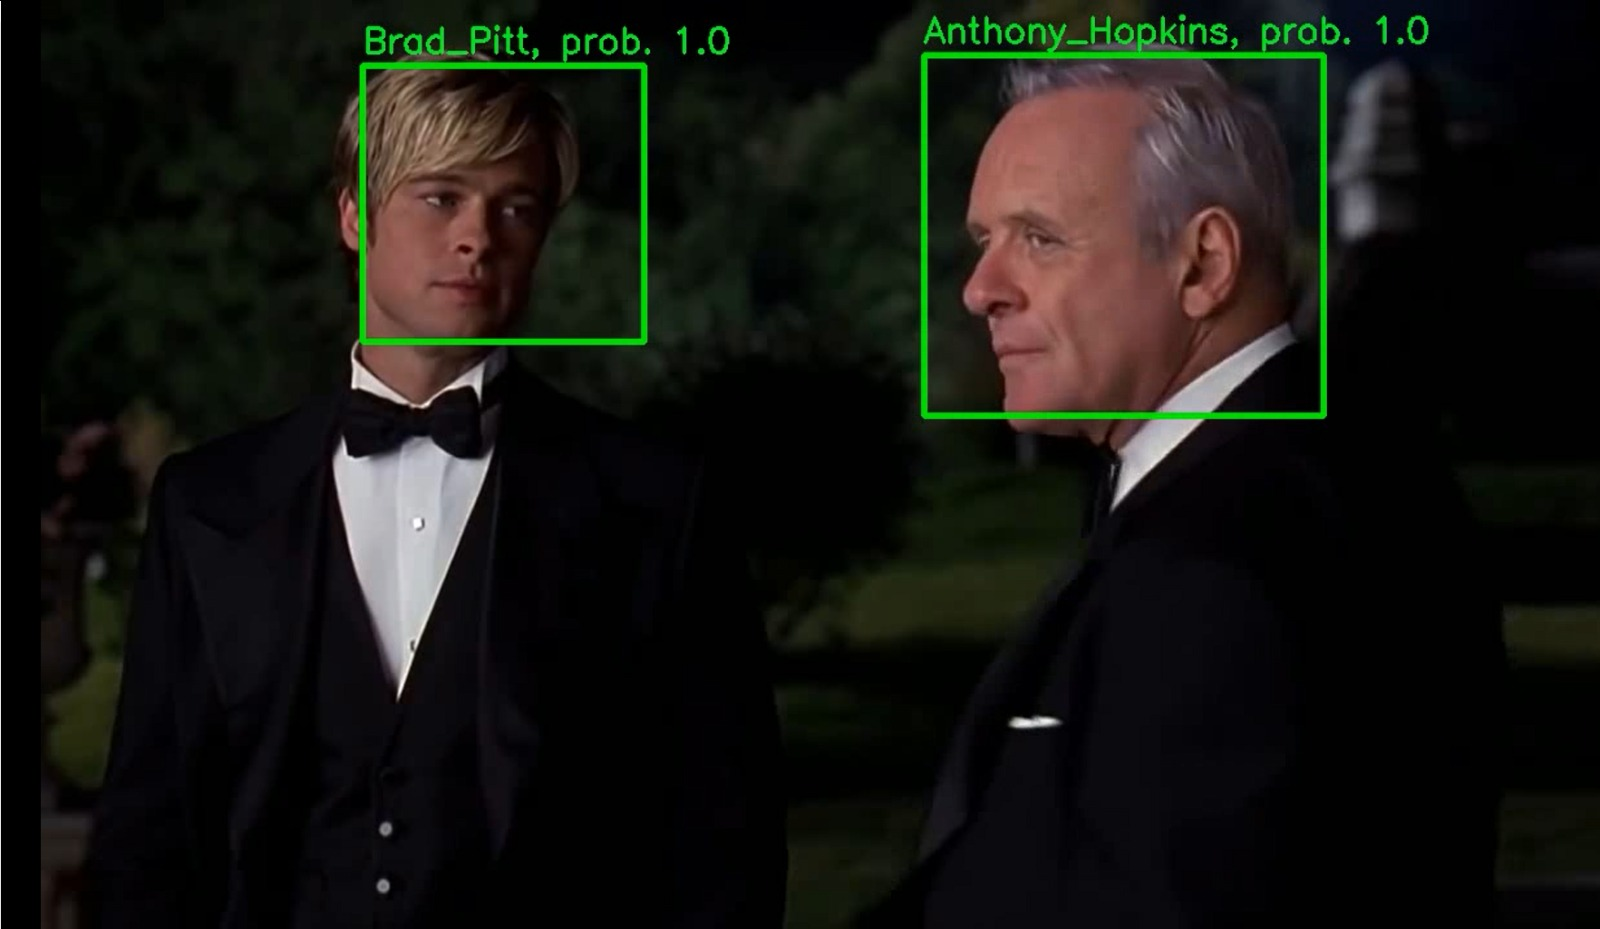
\includegraphics[scale=0.2]{images/demo7.jpeg}  \\
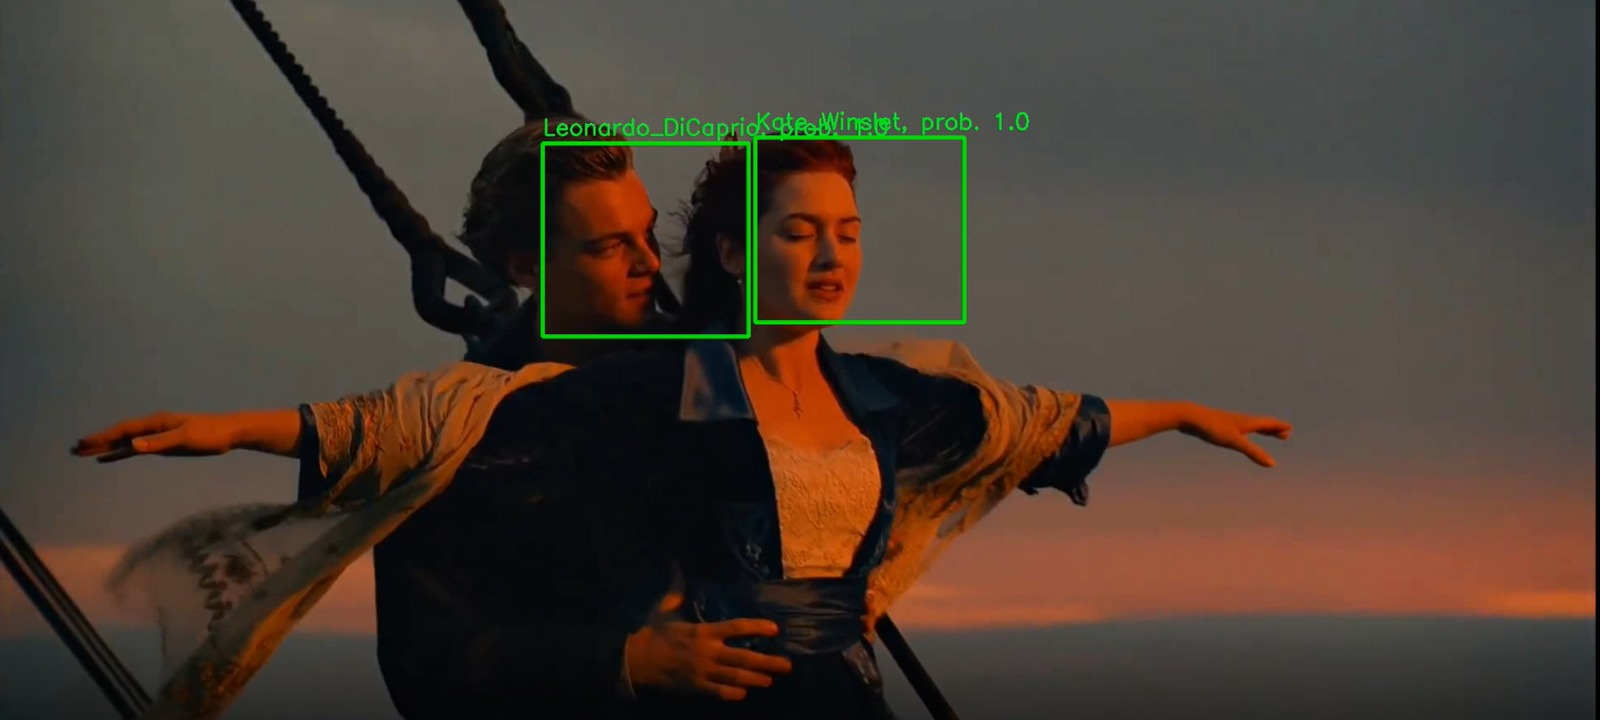
\includegraphics[scale=0.2]{images/demo6.jpeg}\\  
\begin{center}
See full demo on: \url{https://drive.google.com/drive/u/1/folders/1z9Fb8l9Ao-0TQoR09Her3iaGBIrc5KQJ}
\begin{multicols}{4}
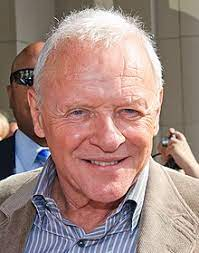
\includegraphics[scale=0.38]{images/Anhony_Hopkins.jpg}
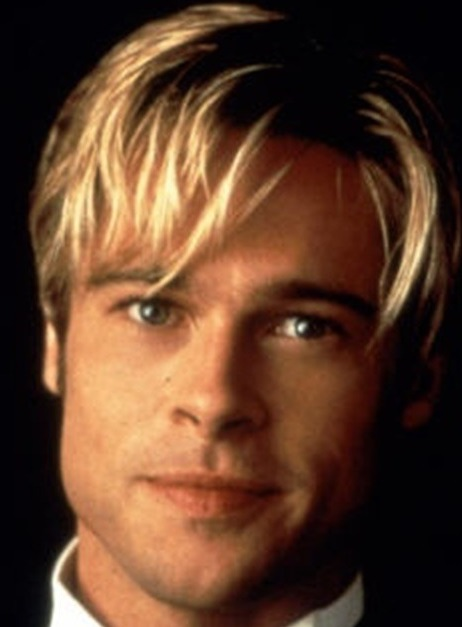
\includegraphics[scale=0.25]{images/Brad_Pitt.jpg}
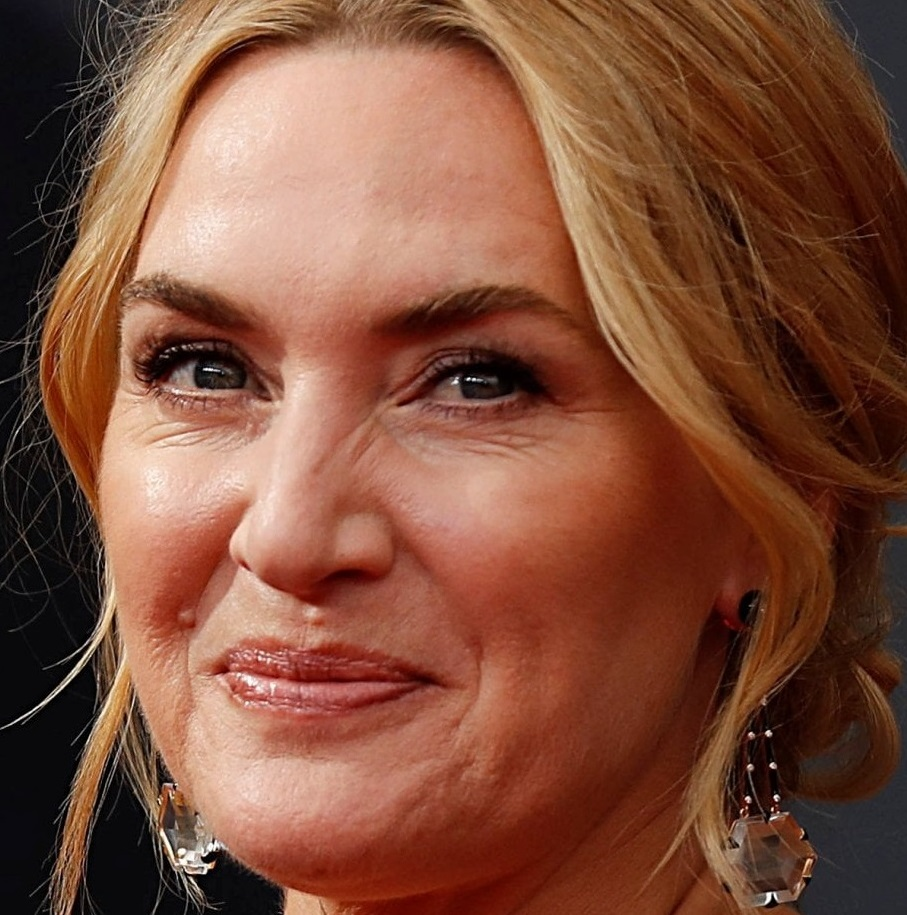
\includegraphics[scale=0.16]{images/Kate_Winslet.jpg}
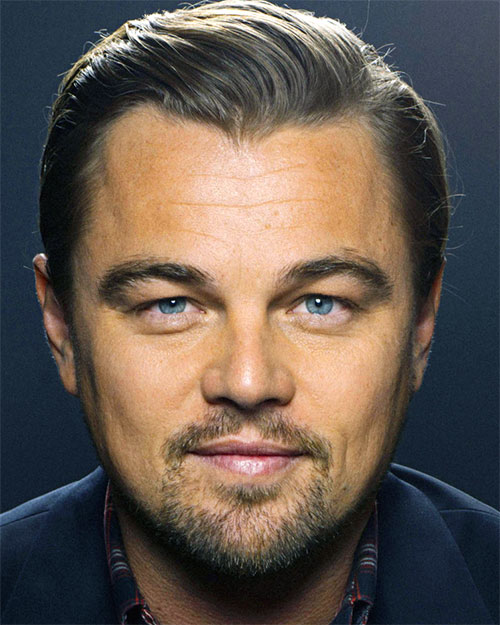
\includegraphics[scale=0.16]{images/Leonardo Di Caprio.jpg}
\end{multicols}
\end{center}    

\end{document}


%%%
Project Milestone
Your project milestone report should be between 2 - 3 pages using the provided template. The following is a suggested structure for your report:
Title, Author(s)
Introduction: this section introduces your problem, and the overall plan for approaching your problem
Problem statement: Describe your problem precisely specifying the dataset to be used, expected results and evaluation
Technical Approach: Describe the methods you intend to apply to solve the given problem
Intermediate/Preliminary Results: State and evaluate your results upto the milestone

Submission: Please submit your milestone as a single PDF on AImageLab Courses. Only one person on your team should submit. You can update your submission before the deadline.
Deadline: There is a strict deadline to submit your project proposal (see the “Important dates” section above).
Grading: The project milestone will contribute to 5 out of 33 points of your final exam grade. Teams who do not submit the project milestone by the deadline will receive 0/5 points.
%%%